\problemname{Galaxy Quest}

%\illustration{0.3}{image.jpg}{Caption of the illustration (optional). CC BY-NC 2.0 by X on Y}
% Source: URL to image.

\newcommand{\maxn}{10^5}
\newcommand{\maxc}{10^3}

You are travelling through the galaxy in your spaceship.
There are $n$ planets in the galaxy, numbered from $1$ to $n$ and modelled as points in $3$-dimensional space.

You can travel between these planets along $m$ space highways, where each highway connects two planets along the straight line between them.
Your engine can accelerate (or decelerate) at $\SI{1}{\metre\per\second\squared}$, while using fuel at a rate of $1$ litre per second.
There is no limit to how fast you can go, but you must always come to a complete
standstill whenever you arrive at the planet at the end of a highway.

It is possible for a highway to pass through planets other than the ones it connects.
However, as your spaceship is equipped with special hyperspace technology, it simply phases through these obstacles without any need of stopping.
Another consequence of using this technology is that it is impossible to jump from one highway to another midway through: highways must always be travelled in full.

\begin{figure}[!h]
  \centering
  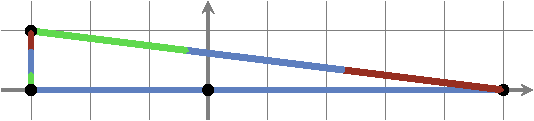
\includegraphics[width=0.6\textwidth]{sample1.pdf}
  \caption{Illustration of Sample Input 1, showing highways in blue, and a
    route from planet $1$ to planet $3$.
    The green start of a highway indicates acceleration,
    and the red end indicates deceleration.}
  \label{fig:galaxy}
\end{figure}

You need to fly several missions, in which you start at your home planet (with number $1$) and need to reach a given target planet within a given time limit.
For each mission, determine whether it can be completed, and if so, find the
least amount of fuel required to do so.
As an example, Figure~\ref{fig:galaxy} shows the optimal route for the second mission of the first sample.

\begin{Input}
  The input consists of:
  \begin{itemize}
    \item One line with three integers $n$, $m$, and $q$ ($1 \le n,m,q \le \maxn$, $n \ge 2$),
      where $n$ is the number of planets, $m$ is the number of space highways, and $q$ is the number of missions.
    \item $n$ lines, each with three integers $x_i$, $y_i$, and $z_i$ ($\left|x_i\right|,\left|y_i\right|,\left|z_i\right| \le \maxc$, $1 \le i \le n$), the coordinates of planet $i$.
    \item $m$ lines, each with two integers $a$ and $b$ ($1 \le a,b \le n$, $a \neq b$), describing a space highway that connects planets $a$ and $b$. It can be traversed in either direction.
    \item $q$ lines, each with two integers $c$ and $t$ ($2 \le c \le n$, $1 \le t \le \maxc$), the target planet and time limit for each mission.
  \end{itemize}
  The $n$ planets are in distinct locations.
  Their coordinates are given in metres, and the time limits of the missions are given in seconds.
  No two highways connect the same pair of planets.
  For each mission, both the absolute and relative differences between the given time limit and the shortest possible completion time are at least $10^{-6}$.
\end{Input}

\begin{Output}
  For each mission, output the least amount of fuel in litres required to reach the target location within the time limit.
  If the target location cannot be reached within the time limit, output ``\texttt{impossible}''.

  Your answers should have an absolute or relative error of at most $10^{-6}$.
\end{Output}
